This section is a general overview to show how easy it is to load
and manipulate data on the file system and over the web using python's
built in data structures and numpy arrays.  The goal is to exercise
basic programming skills like building filename or web addresses to
automate certain tasks like loading a series of data files or
downloading a bunch of related files off the web, as well as to
illustrate basic numpy and pylab skills.

\section{Loading and saving ASCII data}
\label{sec:ascii_data}

The simplest file format is a plain text ASCII file of numbers.
Although there are many better formats out there for saveing and
loading data, this format is extremely common because it has the
advantages of being human readable, and thus will survive the test of
time as the \textit{en vogue} programming languages, analysis
applications and data formats come and go, it is easy to parse, and it
is supported by almost all languages and applications.  

In this exercise we will create a data set of two arrays, the first
one regularly sampled time \textit{t} from 0..2 seconds with 20~ms
time step , and the second one an array \texttt{v} of sinusoidal
voltages corrupted by some noise.  Let's assume the sine wave has
amplitude 2~V, frequency 10~Hz, and zero mean Gaussian distrubuted
white noise with standard deviation 0.5~V.  Your task is to write two
scripts.

The first script should create the vectors \texttt{t} and \texttt{v},
plot the time series of \texttt{t} versus \texttt{v}, save them in a
two dimensional numpy array \texttt{X}, and then dump the array
\texttt{X} to a plain text ASCII file called
\texttt{'noisy\_sine.dat'}.  The file will look like (not identical
because of the noise)

\begin{verbatim}
0.000000000000000000e+00 1.550947826934816025e-02
2.000000000000000042e-02 2.493944587057004725e+00
4.000000000000000083e-02 9.497694074551737975e-01
5.999999999999999778e-02 -9.185779287524413750e-01
8.000000000000000167e-02 -2.811127590689064704e+00
... and so on
\end{verbatim}

Here is the exercise skeleton of the script to create and plot the
data file

\lstinputlisting[label=code:noisy_sine,caption={IGNORED}]{problems/noisy_sine.py}

and the graph will look something like Figure~\ref{fig:noisy_sine}

\begin{center}%
\begin{figure}
\begin{centering}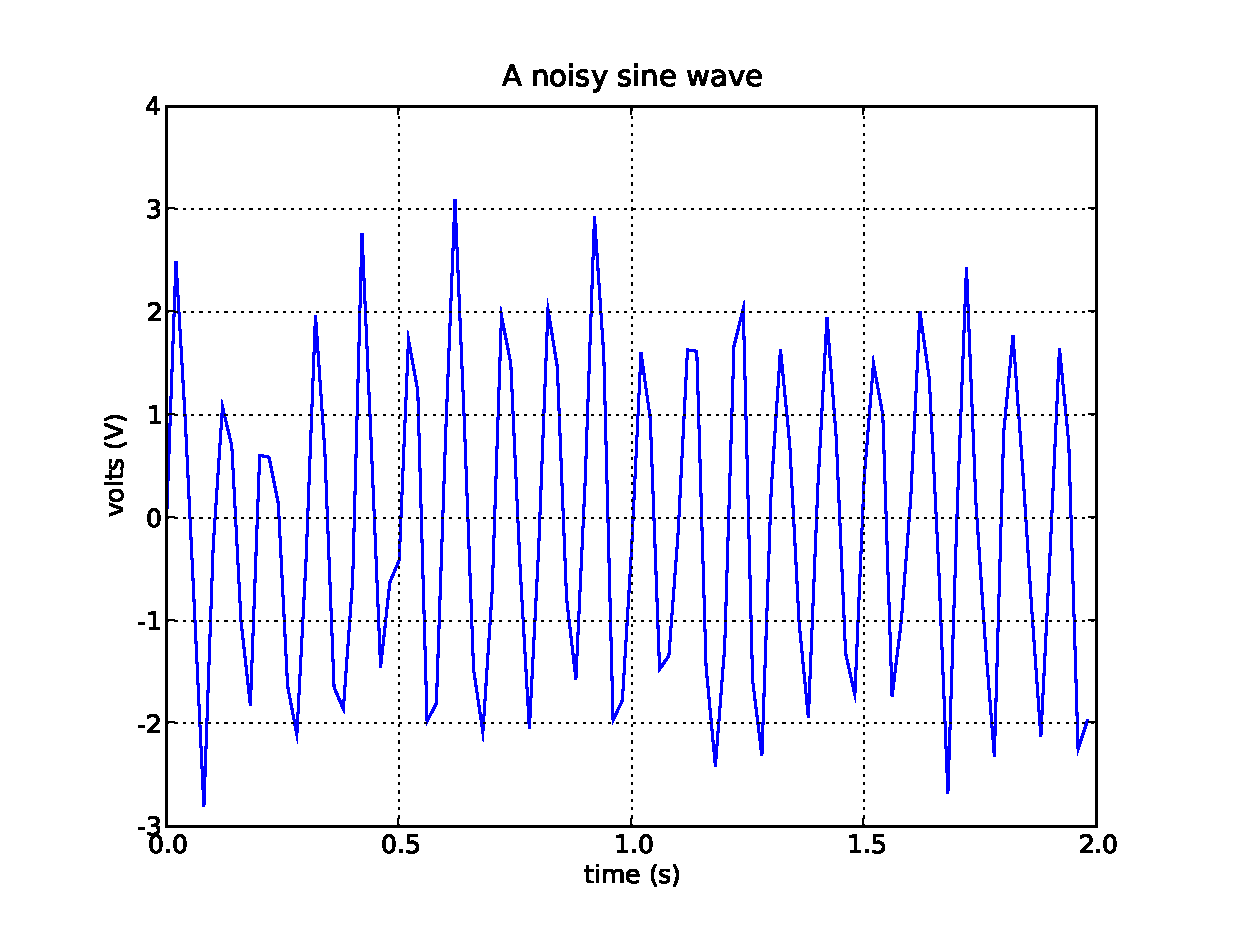
\includegraphics[width=4in]{fig/noisy_sine}\par\end{centering}


\caption{\label{fig:noisy_sine}A 10~Hz sine wave corrupted by noise}
\end{figure}
\par\end{center}


The second part of this exercise is to write a script which loads data
from the data file into an array \texttt{X}, extracts the columns into
arrays \texttt{t} and \texttt{v}, and computes the RMS
(root-mean-square) intensity of the signal using the \texttt{load}
command.

\section{Working with CSV files}

The CSV (Comma Separated Value) file specification is also an ASCII
based, human readable format, but it is more powerful than simple flat
ASCII files including headers, escape sequences and arbitrary
delimiters like TAB, SPACE or COMMA.  It is a widely used interchange
format for sharing data between operating systems and programs like
Excel, Matlab and statistical analysis packages.

A typical CSV file will be a mix of different data types: integers,
floating point numbers, dates and strings.  Of course, all of these
are strings in the file, since all text files are made up of strings,
but the data is typically representing some other numeric or date
type.  Python has very good support for handling different data types,
so you don't need to try to force your data to look like a multi
dimensional array of floating point numbers if this is not the natural
way to describe your data.  numpy provides a generalization of the
array data structure we used above called record arrays, which allow
to store data in a conceptual model similar to a database or
spreadsheet: several named fields (eg 'date', 'weight', 'height',
'age') with different types (eg \texttt{datetime.date}, \texttt{float},
\texttt{float}, \texttt{int}).

In the example below, we will download some CSV files from Yahoo
Financial web pages and load them into numpy record arrays for
analysis and visualization.  Go to \texttt{http://finance.yahoo.com}
and enter a stock symbol in the entry boc labeled ``Get Quotes''.  I
will use \texttt{'SPY'} which is an index fund that tracks the S\&P
500.  In the left menu bar, there is an entry called ``Historical
Prices'' which will take you to a page where you can download the
price history of your stock.  Near the bottom of this page you should
see a ``Download To Spreadsheet'' link -- instead of clicking on it,
right click it and choose ``Copy Link Location'' and paste this into a
python script or ipython session as a string named \texttt{url}.  Eg,
for SPY page better

\begin{lstlisting}
url = 'http://ichart.finance.yahoo.com/table.csv?' +\
   's=SPY&d=9&e=20&f=2007&g=d&a=0&b=29&c=1993&ignore=.csv'
\end{lstlisting}

\noindent I've broken the url into two strings so they will fit on the
page.  If you spend a little time looking at this pattern, you can
probably figure out what is going on.  The URL is encoding the
information about the stock, the variable \texttt{s} for the stock
ticker, \texttt{d} for the latest month, \texttt{e} for the latest
day, \texttt{f} for the latest year, \texttt{c} for the start year,
and so on (similarly \texttt{a}, \texttt{b}, and \texttt{c} for the
start month, day and year).  This is handy to know, because below we
will write some code to automate some downloads for a stock universe.

One of the great things about python is it's ``batteries included''
standard library, which includes support for dates, csv files and
internet downloads.  The example interactive session below shows how
in just a few lines of code using python's \texttt{urllib} for
retrieving information from the internet, and matplotlib's
\texttt{csv2rec} function for loading numpy record arrays, we are
ready to get to work analyzing some web based data.  Comments have
been added to a copy-and-paste from the interactive session

\begin{lstlisting}
# import a couple of libraries we'll be needing
In [23]: import urllib
In [24]: import matplotlib.mlab as mlab

# this is the CSV file we'll be downloading
In [25]: url = 'http://ichart.finance.yahoo.com/table.csv?' +\
   's=SPY&d=9&e=20&f=2007&g=d&a=0&b=29&c=1993&ignore=.csv'

# this will grab that web file and save it as 'SPY.csv' on our local
# filesystem
In [27]: urllib.urlretrieve(url, 'SPY.csv')
Out[27]: ('SPY.csv', <httplib.HTTPMessage instance at 0x2118210>)

# here we use the UNIX command head to peak into the file, which is
# a comma separated and contains various types, dates, ints, floats
In [28]: !head SPY.csv
Date,Open,High,Low,Close,Volume,Adj Close
2007-10-19,153.09,156.48,149.66,149.67,295362200,149.67
2007-10-18,153.45,154.19,153.08,153.69,148367500,153.69
2007-10-17,154.98,155.09,152.47,154.25,216687300,154.25
2007-10-16,154.41,154.52,153.47,153.78,166525700,153.78
2007-10-15,156.27,156.36,153.94,155.01,161151900,155.01
2007-10-12,155.46,156.35,155.27,156.33,124546700,156.33
2007-10-11,156.93,157.52,154.54,155.47,233529100,155.47
2007-10-10,156.04,156.44,155.41,156.22,101711100,156.22
2007-10-09,155.60,156.50,155.03,156.48,94054300,156.48

# csv2rec will import the file into a numpy record array, inspecting
# the columns to determine the correct data type
In [29]: r = mlab.csv2rec('SPY.csv')

# the dtype attribute shows you the field names and data types.  
# O4 is a 4 byte python object (datetime.date), f8 is an 8 byte 
# float, i4 is a 4 byte integer and so on.  The > and < symbols
# indicate the byte order of multi-byte data types, eg big endian or
# little endian, which is important for cross platform binary data
# storage
In [30]: r.dtype
Out[30]: dtype([('date', '|O4'), ('open', '>f8'), ('high', '>f8'),
('low', '>f8'), ('close', '>f8'), ('volume', '>i4'), ('adj_close',
'>f8')])

# Each of the columns is stored as a numpy array, but the types are 
# preserved.  Eg, the adjusted closing price column adj_close is a
# floating  point type, and the date column is a python datetime.date
In [31]: print r.adj_close
[ 149.67  153.69  154.25 ...,   34.68   34.61   34.36]
In [32]: print r.date
[2007-10-19 00:00:00 2007-10-18 00:00:00 2007-10-17 00:00:00 ...,
 1993-02-02 00:00:00 1993-02-01 00:00:00 1993-01-29 00:00:00]
\end{lstlisting}

For your exercise, you'll elaborate on the code here to do a batch
download of a number of stock tickers in a defined stock universe.
Define a function \texttt{fetch\_stock(ticker)} which takes a stock
ticker symbol as an argument and returns a numpy record array.  Select
the rows of the record array where the date is greater than 2003-01-01
and plot the returns $(p-p_0)/p_0$ where $p$ are the prices and $p_0$
is the initial price. by date for each stock on the same plot.  Create
a legend for the plot using the matplotlib \texttt{legend} command,
and print out a sorted list of final returns (eg assuming you bought
in 2003 and held to the present) for each stock.  Here is the exercise
skeleton.:

\lstinputlisting[label=code:stock_records,caption={IGNORED}]{problems/stock_records.py}

The graph will look something like Figure~\ref{fig:stock_records}.

\begin{center}%
\begin{figure}
\begin{centering}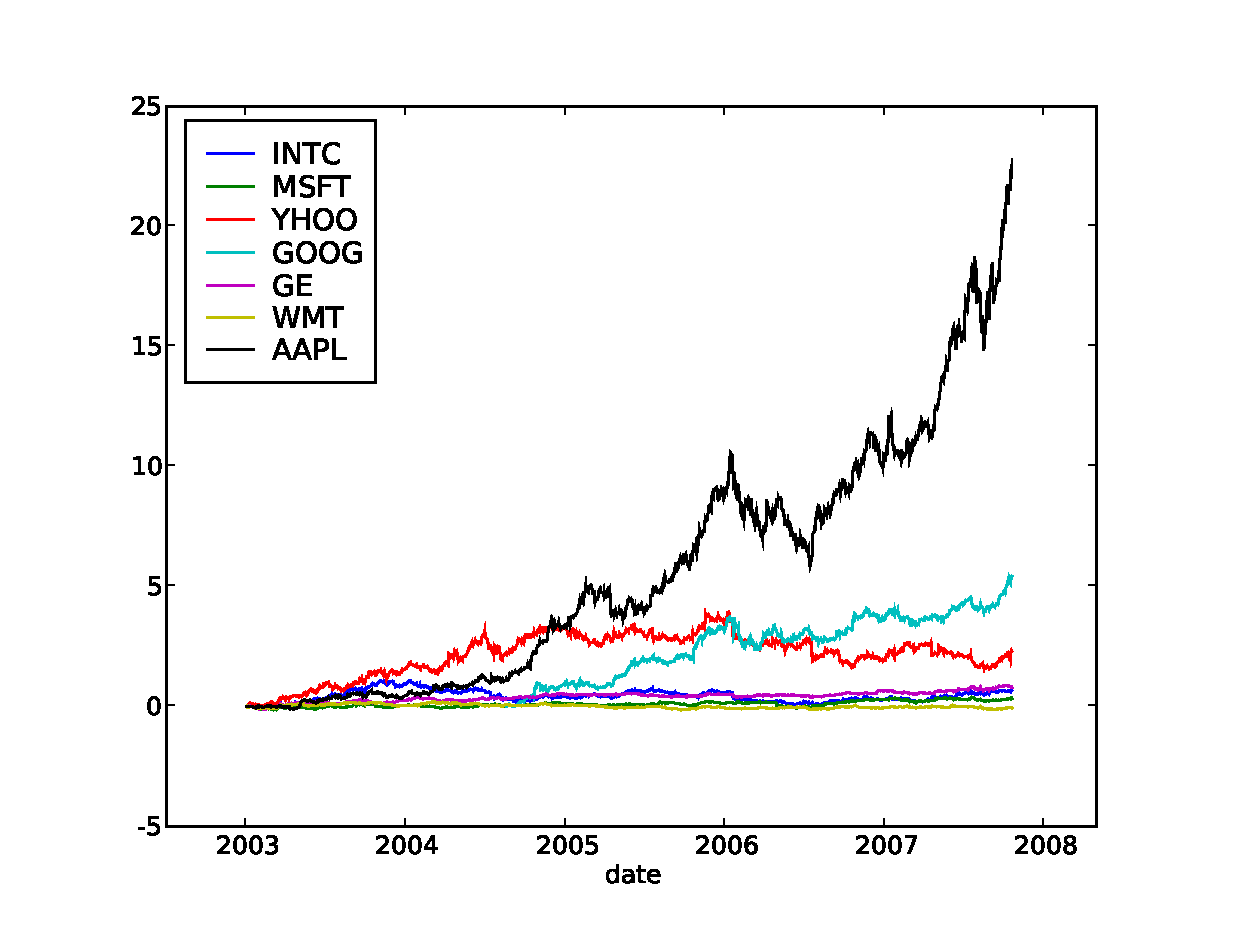
\includegraphics[width=4in]{fig/stock_records}\par\end{centering}


\caption{\label{fig:stock_records}Returns for a universe of stocks
  since 2003}
\end{figure}
\par\end{center}


\section{Loading and saving binary data}
\label{sec:binary_data}

ASCII is bloated and slow for working with large arrays, and so binary
data should be used if performance is a consideration.  To save an
array \texttt{X} in binary form, you can use the numpy
\texttt{tostring} method

\begin{lstlisting}
In [16]: import numpy

# create some random numbers
In [17]: x = numpy.random.rand(5,2)

In [19]: print x
[[ 0.56331918  0.519582  ]
 [ 0.22685429  0.18371135]
 [ 0.19384767  0.27367054]
 [ 0.35935445  0.95795884]
 [ 0.37646642  0.14431089]]

# save it to a data file in binary
In [20]: x.tofile(file('myx.dat', 'wb'))

# load it into a new array
In [21]: y = numpy.fromfile(file('myx.dat', 'rb'))

# the shape is not preserved, so we will have to reshape it
In [22]: print y
[ 0.56331918  0.519582    0.22685429  0.18371135  0.19384767
0.27367054
  0.35935445  0.95795884  0.37646642  0.14431089]

In [23]: y.shape
Out[23]: (10,)

# restore the original shape
In [24]: y.shape = 5, 2

In [25]: print y
[[ 0.56331918  0.519582  ]
 [ 0.22685429  0.18371135]
 [ 0.19384767  0.27367054]
 [ 0.35935445  0.95795884]
 [ 0.37646642  0.14431089]]
\end{lstlisting}

The advantage of numpy \texttt{tofile} and \texttt{fromfile} over
ASCII data is that the data storage is compact and the read and write
are very fast.  It is a bit of a pain that that meta ata like array
datatype and shape are not stored.  In this format, just the raw binary
numeric data is stored, so you will have to keep track of the data
type and shape by other means.  This is a good solution if you need to
port binary data files between different packages, but if you know you
will always be working in python, you can use the python pickle
function to preserve all metadata (pickle also works with all standard
python data types, but has the disadvantage that other programs and
applications cannot easily read it)

\begin{lstlisting}
# create a 6,3 array of random integers
In [36]: x = (256*numpy.random.rand(6,3)).astype(numpy.int)

In [37]: print x
[[173  38   2]
 [243 207 155]
 [127  62 140]
 [ 46  29  98]
 [  0  46 156]
 [ 20 177  36]]

# use pickle to save the data to a file myint.dat
In [38]: import cPickle

In [39]: cPickle.dump(x, file('myint.dat', 'wb'))

# load the data into a new array
In [40]: y = cPickle.load(file('myint.dat', 'rb'))

# the array type and share are preserved
In [41]: print y
[[173  38   2]
 [243 207 155]
 [127  62 140]
 [ 46  29  98]
 [  0  46 156]
 [ 20 177  36]]
\end{lstlisting}



